\documentclass[journal]{IEEEtran}

\usepackage{cite}
\usepackage[pdftex]{graphicx}
\usepackage{float}
\usepackage{amssymb}
\usepackage{amsmath}

\begin{document}


\title{Optimization}

\author{Rodrigo Caye Daudt}

% The paper headers
\markboth{Optimization}%
{Rodrigo Caye Daudt}


% make the title area
\maketitle


\begin{abstract}
%\boldmath
This describes the implementation and results of several minimization/optimization methods. The methods are divided in three groups: 1D, 2D, and ND inputs.
\end{abstract}




\IEEEpeerreviewmaketitle


%%%%%%%%%%%%%%%%%%%%%%%%%%%%%%%%%%%%%%%%%%%%%%%%%%%%%%%%%%%%%%%%%%%%%%%%%%%%%%%%
%%%%%%%%%%%%%%%%%%%%%%%%%%%%%%%%%%%%%%%%%%%%%%%%%%%%%%%%%%%%%%%%%%%%%%%%%%%%%%%%
\section{Introduction}

\IEEEPARstart{F}{unction} optimization is a field of mathematics that deals with the search of the input element of a function that yields the output that best conforms with some predefined criteria. This seach has many applications throughout different scientific fields, from economics to control engineering. Some applications of function minimization are the training of neural networks, simultaneos localization and mapping (SLAM), and real time optimization (RTO) control.

Several different methods of function optimization are presented in the following sections. These methods are described and compared, focusing on pratical aspects such as complexity, convergence issues and issues with logal minima.




%%%%%%%%%%%%%%%%%%%%%%%%%%%%%%%%%%%%%%%%%%%%%%%%%%%%%%%%%%%%%%%%%%%%%%%%%%%%%%%%
%%%%%%%%%%%%%%%%%%%%%%%%%%%%%%%%%%%%%%%%%%%%%%%%%%%%%%%%%%%%%%%%%%%%%%%%%%%%%%%%
\section{Code Glossary}

The code that was used to exemplify and evaluate the optimization methods presented later in this paper were programmed using MATLAB. The files can be divided in three groups: functions to be minimized, functions used in the minimization process and scripts. Next is a glossary of the files contained in this work.

Scripts:
\begin{itemize}
    \item Part1.m - This script exemplifies the optimization methods of functions with 1 dimensional inputs.
    \item Part2.m - This script exemplifies the optimization methods of functions with 2 dimensional inputs.
    \item Part3.m - This script exemplifies the optimization methods of functions with N dimensional inputs.
\end{itemize}

Functions to be minimized:
\begin{itemize}
    \item f1.m - Example of 1 dimensional input function.
    \item 21.m - Example of 2 dimensional input quadratic form.
    \item f2-2.m - Goldstein-Price function.
    \item dtF.m - Total cost function for ellipse fitting with Levenberg-Marquardt method.
\end{itemize}

Functions used in the minimization operations:
\begin{itemize}
    \item dtBrent.m - Brent's method minimizer of any N-dimensional function along a given direction.
    \item dtGrad.m - Numerical calculation of an N-dimensional function's gradient vector.
    \item dtHess2d.m - Numerical calculation of a 2-dimensional function's Hessian matrix.
    \item dtError.m - Cost function for a given point used for fitting an ellipse.
    \item dtEllipse\_noisy.m - Generates noisy samples for an ellipse with the given parameters.
    \item dtEllipse.m - Generates sequential points with no added noise along the perimeter of the ellipse with the given parameters for plotting.
\end{itemize}

The code can be found at \cite{github}.

%%%%%%%%%%%%%%%%%%%%%%%%%%%%%%%%%%%%%%%%%%%%%%%%%%%%%%%%%%%%%%%%%%%%%%%%%%%%%%%%
%%%%%%%%%%%%%%%%%%%%%%%%%%%%%%%%%%%%%%%%%%%%%%%%%%%%%%%%%%%%%%%%%%%%%%%%%%%%%%%%
\section{Minimization In 1D} \label{1d}

To follow a roughly increasing order of complexity in the tested algorithms, the first examples are minimizations of $\mathbb{R}\rightarrow\mathbb{R}$ functions. The fuction that was minimized in the following examples was:

\begin{equation}
f(x) = e^{-(x+1)^2}-e^{-x^2}
\label{f1}
\end{equation}

This function has its global minimum at $x\approx 0.2717$, where $f(x)\approx -0.7304$. This function has no other local minima.

%%%%%%%%%%%%%%%%%%%%%%%%%%%%%%%%%%%%%%%%%%%%%%%%%%%%%%%%%%%%%%%%%%%%%%%%%%%%%%%%
\subsection{Brute Force}

The first implemented method is the most intuitive and the simplest to understand. The brute force method finds the minimum of the function by sampling a very big amount of points, applying the function to those points and comparing the results. The precision of the result can be controlled by the amount of samples that are calculated in the process.

Figure \ref{figBF} shows a plot of the function described in Eq. \ref{f1} along with the identification of the calculated minimum. The function was evaluated at 20001 points between -10 and 10. The minimum obtained by this method was $x = 0.2717$, which is the correct value.

\begin{figure}[H]
\centering
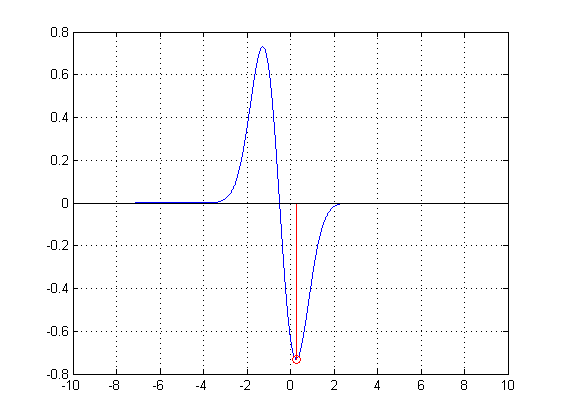
\includegraphics[width=3.4in]{figures/1d-bruteForce.png}
\caption{Brute Force}
\label{figBF}
\end{figure}

This method is very reliable and easy to program, but it's the most complex method for the computer to calculate. Another advantage of this method is that it is immune to local minima in the interval it analyses, since it evaluate "all" the points in that interval. The precision of the obtained value increases slowly with the number of points used in the calculation, that is, to increase the precision by a factor of $c$ we need to use $c$ times more points, which makes this method undesirable for most applications.

%%%%%%%%%%%%%%%%%%%%%%%%%%%%%%%%%%%%%%%%%%%%%%%%%%%%%%%%%%%%%%%%%%%%%%%%%%%%%%%%
\subsection{Golden Search}

The golden search optimization method needs three points to start its calculations. Firstly, it's necessary checking there is a minimum in the range defined by these points by checking if the function evaluated at the middle point is smaller than the function evaluated at the outer points. If so, a new point is chosen (preferably inside the largest interval) and the function is evaluated at this point. The result defines which three points will be kept for the next iteration, and the process is applied again over a smaller interval. This process stops when a maximum number of iteration is reached or if a predefined precision is acheved, that is, the distance between the outer points is smaller than a desired threshold.

 This method, as was described above, is iterative. This makes its convergence much faster than the brute force method, which means less calculations are needed for a given precision to be achieved. Also, if a greater precision is desired, all that has to be done is to add a few iterations to further approximate the result.

Figure \ref{figGS} shows the central point of several iterations of the golden search method when applied to the function described in Eq. \ref{f1}. We can easily observe the fast rate of convergence when compared to the brute force method. In the presented case, the method started from the points $x_1=-10$, $x_2=-0.4$ and $x_3=10$. It reached the same result of the brute force method, $x = 0.2717$. The method took 29 iterations to achieve a precision of $\epsilon = 0.00001$.

\begin{figure}[H]
\centering
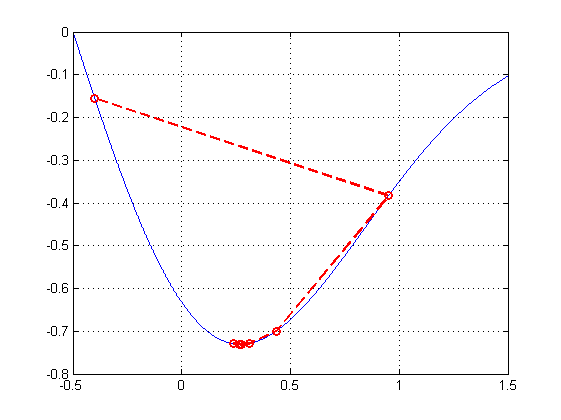
\includegraphics[width=3.4in]{figures/1d-goldenSearch.png}
\caption{Golden Search}
\label{figGS}
\end{figure}

The golden search method is completely stable as long as the initial points are guaranteed to contain a minimum in the interval they define. The main issue with this method is the initial choice of points for the first iteration of the algorithm. Given an appropriate set of starting points, this method will find a minimum in the defined interval, but the minimum it finds can be a local minimum instead of the real minimum in the interval.

%%%%%%%%%%%%%%%%%%%%%%%%%%%%%%%%%%%%%%%%%%%%%%%%%%%%%%%%%%%%%%%%%%%%%%%%%%%%%%%%
\subsection{Brent's Method}

The next optimization method to be applied to 1D functions was Brent's method. This method has a lot in common with the golden search method. It begins with three points that define a range with at least one minimum. The main difference between these two methods is the choice of the new point to be analysed. While in the golden search the new point is chosen solely based on the abscissas of the current 3 points, Brent's method takes into account the ordinate of the function at these points and interpolates a parabola along these points to estimate where the minimum is.

This usage of information from the function itself generally leads Brent's method to a faster convergence in terms of iterations. It tends to work even better the closer the current guesses are, as long as the function is well behaved in this area and can be approximated by a curve, which is true in most situations.

Figure \ref{figBM} shows the central point of several iterations of Brent's method when applied to the function described in Eq. \ref{f1}. The result obtained by this method was exactly the same as the one obtained through brute force and golden search, but Brent's method took only 18 iterations to achieve a precision of $\epsilon = 0.00001$.

\begin{figure}[H]
\centering
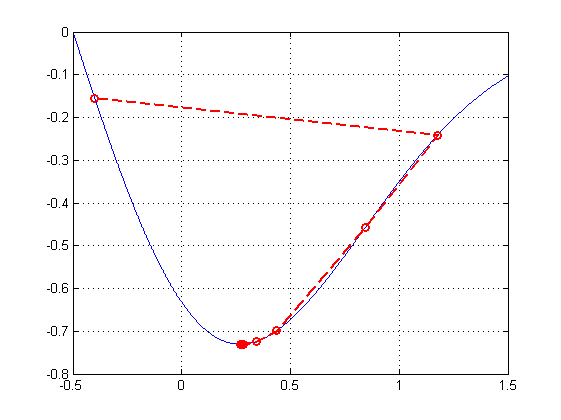
\includegraphics[width=3.4in]{figures/1d-brentsMethod.png}
\caption{Brent's Method}
\label{figBM}
\end{figure}

Just as in the golden search method, Brent's method stability is guaranteed as long as the initial points satisfy the $$f(a)>f(b)<f(c)$$ condition. Since the complexity of Brent's method and the golden search method are very similar, they are stable in the same cases, and Brent's method converges faster, Brent's method was considered superior to the golden search method in these tests.

%%%%%%%%%%%%%%%%%%%%%%%%%%%%%%%%%%%%%%%%%%%%%%%%%%%%%%%%%%%%%%%%%%%%%%%%%%%%%%%%
\subsection{Gauss-Newton Method}

The Gauss-Newton approach for function optimization takes a different route than the previous methods to find the optimum point of the function. This method only takes a single point to start from. It then calculates the first and second derivatives of the function at that point, and calculates the next point according to the formula below.

$$x_{n+1} = x_n - \frac{f'(x)}{f''(x)}$$ \cite{yohan}

The algorithm continues to calculate new values of $x_n$ until the difference between the new value and the current value is below a predefined threshold, or if the number of iterations reaches a limit. If the value of $x_n$ ctops changing significantly it means that the first derivative of the function at the current point is very close to 0, and is considered an extremum.

Figure \ref{figGN} shows an example of the points obtained by the calculations following the Gauss-Newton method. We can observe that this method converges quickly when it's close to the extremum, but it may be erratic far from it. This method took 7 iterations to converge to a precision of $\epsilon = 0.00001$ when starting from $x = -0.3$.

\begin{figure}[H]
\centering
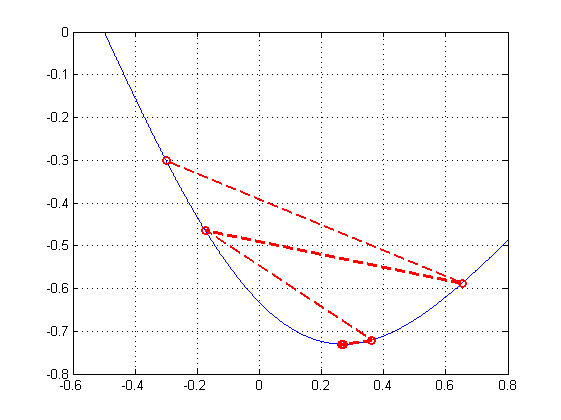
\includegraphics[width=3.4in]{figures/1d-newtonsMethod.png}
\caption{Gauss-Newton Method}
\label{figGN}
\end{figure}

The Gauss-Newton method has several limitations. First, its convergence is never certain, so the search for an extremum may not have any relevant results. Another problem with this method is that it doesn't discern between maxima and minima, so even if the algorithm reaches a point of equilibrium that point may not be what we are looking for. Finally, this method is also sensible to local minima and maxima. All these characteristics must be taken into account when applying this method on a real optimization.


%%%%%%%%%%%%%%%%%%%%%%%%%%%%%%%%%%%%%%%%%%%%%%%%%%%%%%%%%%%%%%%%%%%%%%%%%%%%%%%%
%%%%%%%%%%%%%%%%%%%%%%%%%%%%%%%%%%%%%%%%%%%%%%%%%%%%%%%%%%%%%%%%%%%%%%%%%%%%%%%%
\section{Minimization Of A Quadratic Form In 2D} \label{2d}

Function optimization in 2D requires more advanced methods than function optimization in 1D, but it also creates oportunities to use more elaborate ideas. In higher dimensions, the brute force method scales poorly since we would need exponentially more samples as the number of dimensions goes up to keep the same precision in the result.

Many of the methods for 2D minimization that will be presented here use an "ideal 1D minimizer" in its algorithm. In our situation there is no such thing, so it was needed to create a function that worked similarly to such an ideal minimizer. By observing the methods shown in Section \ref{1d} and their performances, Brent's method was selected to be applied as our 1D minimizer. Brent's method was chosen because it provided us with the best balance between rate of convergence and stability.

Our 1D minimizer takes as the input the current point, the direction of minimization and the function to be minimized. To apply Brent's method it was first necessary to create other two points that fulfilled the $f(a)>f(b)<f(c)$ requirement. This was done by trying numerous times to generate random points to each side of the input point at increasing distances. Once a set of points fulfilled the basic requirement, Brent's method was applied on this set of points to find a local minimum.

This approximation of an ideal 1D minimizer worked in the vast majority of the presented cases. Given that it generated random points around the central point, each run of this minimizer could incur in a different result, but this was not observed during its application on a quadratic function. This will be further discussed in Section \ref{2d2}.

The quadratic function used in the examples below is described in Eq. \ref{f2}. This function has a minimum at $(x,y)\approx (-0.2174,0.1304)$, where $f(x,y)\approx 3.8261$.

\begin{equation}
f(x,y) = 2*x^2 + 3*y^2 + x*y + x + y + 4
\label{f2}
\end{equation}

%%%%%%%%%%%%%%%%%%%%%%%%%%%%%%%%%%%%%%%%%%%%%%%%%%%%%%%%%%%%%%%%%%%%%%%%%%%%%%%%
\subsection{Arbitrary Line Search}

The arbitrary line search optimization method in 2 dimensions takes as input a starting point and two non-paralel directions. The function is first optimized with an ideal 1D minimizer along the first direction, then it is optimized from the new point along the second direction. This process is repeated until the desired precision is achieved or a maximum number of iterations is reached.

In Fig. \ref{figALS} we can observe an example of the arbitrary line search method being applied to minimize the function described in Eq. \ref{f2}. We can observe that each step is taken in a perpendicular direction. That happens because the directions of minimization used in this example were the directions of each axis.

Starting from the point $(x,y) = (1.5,1.5)$ this method took 10 iteration steps (5 in each direction) to converge to a precision of $\epsilon = 0.00001$. It is important to observe that each step in this minimization process contained a whole 1D minimization, therefore many more hidden calculations take place.

\begin{figure}[H]
\centering
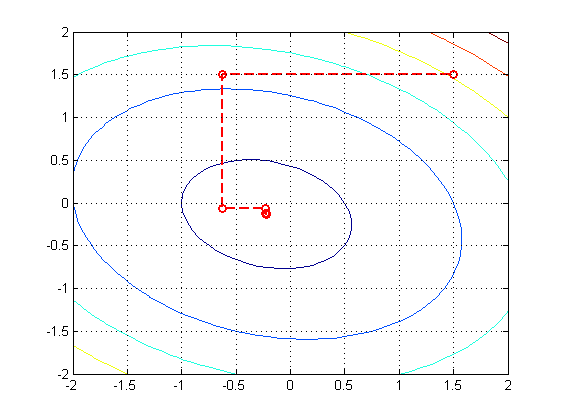
\includegraphics[width=3.4in]{figures/2d-arbitraryLineSearch.png}
\caption{Arbitrary Line Search}
\label{figALS}
\end{figure}

%%%%%%%%%%%%%%%%%%%%%%%%%%%%%%%%%%%%%%%%%%%%%%%%%%%%%%%%%%%%%%%%%%%%%%%%%%%%%%%%
\subsection{Steepest Descent}

The steepest descent method starts from a given point and proceeds to minimize the function along the line than contains the current point and is in the direction of the gradient of the function at that point. This process uses knowledge of the function variation to try to converge faster towards an optimum point.

As is to be expected, the steepest descent method converged faster than the arbitrary line search method in our tests. This faster convergence can be attributed to a smart choice of minimization direction on each point. While the directions of minimization in the arbitrary line search are static throughout the whole process, the minimization directions can change freely on each iteration step (especially when this process is applied for the minimization of functions of higher dimensions). 

Figure \ref{figSD} shows an example of steepest descent optimization of function \ref{f2}. We can observe that the first step, just like every other step, is taken in a perpendicular direction to the level curve at that point since that is the direction of the gradient of the function at that point.

\begin{figure}[H]
\centering
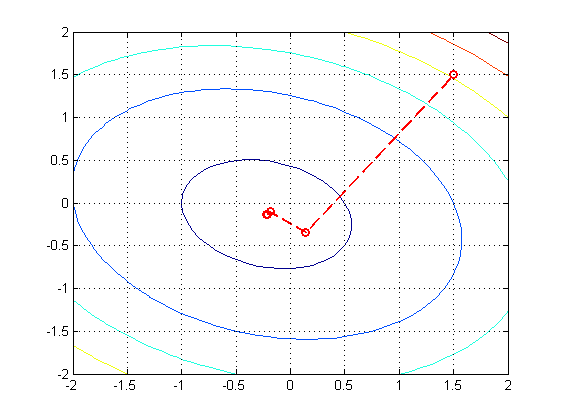
\includegraphics[width=3.4in]{figures/2d-steepestDescent.png}
\caption{Steepest Descent}
\label{figSD}
\end{figure}

Starting from the point $(x,y) = (1.5,1.5)$ this method took 6 iteration steps (5 in each direction) to converge to a precision of $\epsilon = 0.00001$, 4 iterations less than the arbitrary line search method.

%%%%%%%%%%%%%%%%%%%%%%%%%%%%%%%%%%%%%%%%%%%%%%%%%%%%%%%%%%%%%%%%%%%%%%%%%%%%%%%%
\subsection{Powell's Method}

Powell's method takes as input a starting point and two non-parallel minimization directions. At each iteration step, three minimizations occur:

\begin{itemize}
    \item The first one one is along the fist diretion of optimization.
    \item The second one one is along the second diretion of optimization.
    \item The third one is along the direction defined by the starting point and the point obtained after the second minimization.
\end{itemize}

After these steps are taken, the two directions are updated to include the last direction of minimization and then the process is repeated until the desired precision is achieved or a maximum number of iterations is reached. This update in the minimization direction includes the trend in the general direction the function is being updated and this generally leads to a faster convergence of the function.

Figure \ref{figPM} shows the resulting points obtained through Powell's method for minimizing function \ref{f2}, starting from $(x,y) = (1.5,1.5)$ and with the initial directions being the axis directions. This method took 9 iteration steps (3 whole cycles) to converge to a precision of $\epsilon = 0.00001$. This means that in this case it performed slightly better than the arbitrary line search, but was still inferior to the steepest descent method.

\begin{figure}[H]
\centering
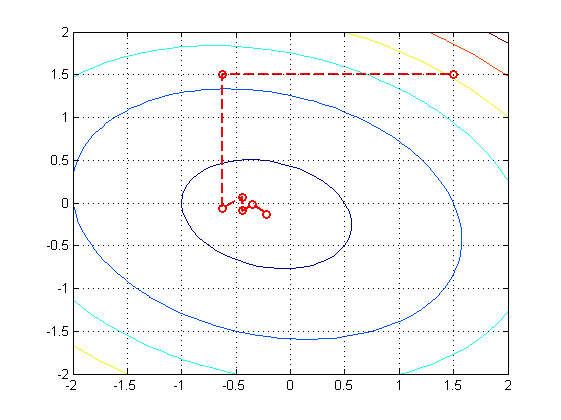
\includegraphics[width=3.4in]{figures/2d-powellsMethod.png}
\caption{Powell's Method}
\label{figPM}
\end{figure}

%%%%%%%%%%%%%%%%%%%%%%%%%%%%%%%%%%%%%%%%%%%%%%%%%%%%%%%%%%%%%%%%%%%%%%%%%%%%%%%%
\subsection{Conjugate Gradient Method}

The conjugate gradient method is an iterative optimization process that tries to approximate the function to a quadratic form. It uses the gradient and the hessian of the function at the current point to try to predict where the minimum will occur. When applied to a quadratic form in 2 dimensions, this method finds the minimum in 2 iterations. This method is by far the most adequate for this situation, eince we are dealing exactly with the minimization of a quadratic function.

Several variations of this method exist and serve best in different situations. For this work it was chosen to implement the "Nonlinear Conjugate Gradients with Newton-Raphson and Fletcher-Reeves" variation\cite{shewchuk1994introduction}. This choice was appropriate since it can be applied numerically to an unknown function without the need to put the function in the quadratic form. This allows for the application of this process to any kind of function and not just quadratics, and this is preferable over other limited variations.

Figure \ref{figCG} shows the iteration steps taken by this method to reach the minimum of the function. The program took 3 iterations to stop. One extra iteration was calculated compared to the theoretical expected value (2 iterations) because one iteration is needed to verify whether the function can be further minimized (this is how the program tells if it has reached a minimum point).

\begin{figure}[H]
\centering
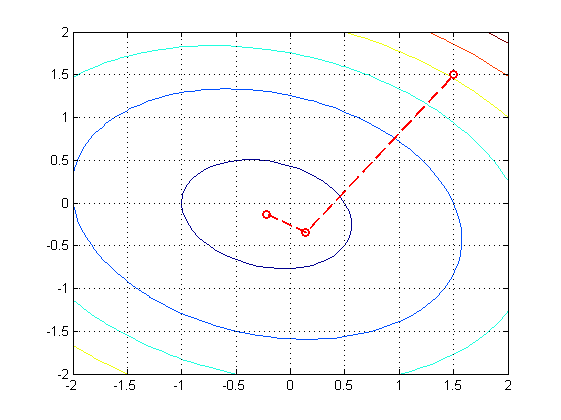
\includegraphics[width=3.4in]{figures/2d-conjugateGradient.png}
\caption{Conjugate Gradient Method}
\label{figCG}
\end{figure}


%%%%%%%%%%%%%%%%%%%%%%%%%%%%%%%%%%%%%%%%%%%%%%%%%%%%%%%%%%%%%%%%%%%%%%%%%%%%%%%%
\section{Goldstein-Price Function Optimization} \label{2d2}

The Goldstein-Price function is used to test the stability of minimization methods. This function is defined in \ref{f22} with $x,y \in [-2,2]$, and has its minimum at $(x,y) = (0,-1)$, where $f(x,y)= 3$.

\begin{equation}
\begin{split}
f(x,y) = (1+((x+y+1)^2)(19-14x+3x^2-14y+\\
+6xy+3y^2))(30+((2x-3y)^2)(18-32x+\\
+12x^2+48y-36xy+27y^2))
\end{split}
\label{f22}
\end{equation}

This function was a much harder challenge for the optimization algorithms since it has several local minima, changes in behaviour rapidly and reaches very high values in its gradient.

%%%%%%%%%%%%%%%%%%%%%%%%%%%%%%%%%%%%%%%%%%%%%%%%%%%%%%%%%%%%%%%%%%%%%%%%%%%%%%%%
\subsection{Arbitrary Line Search}

The arbitrary line search method that was applied here is identical to the one describet in Section \ref{2d}. This method performed fairly well in minimizing the Goldstein-Price function. Starting from the point $(x,y) = (-2,-2)$, this method took 98 iterations to reach a result, but the result it reached was the expected minimum. This suggests this method, although slower to converge than some others, is a very stable method for minimizing 2D functions.

A plot of the results can be seen in Fig. \ref{figALS2}. It seems to follow a vally of the function until it reaches the real minimum point. This image suggests that a better choice of minimization directions could lead to a faster optimization, but prior knowledge about the function being minimized is not always possible and thir result illustrates an optimization without prior knowledge. It should be noted here that not all initial conditions led to the expected minimum, so the stability if this method is still not ideal.

\begin{figure}[H]
\centering
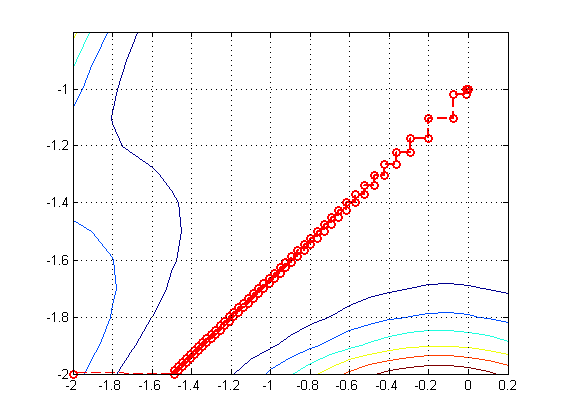
\includegraphics[width=3.4in]{figures/2d2-arbitraryLineSearch.png}
\caption{Arbitrary Line Search}
\label{figALS2}
\end{figure}

%%%%%%%%%%%%%%%%%%%%%%%%%%%%%%%%%%%%%%%%%%%%%%%%%%%%%%%%%%%%%%%%%%%%%%%%%%%%%%%%
\subsection{Steepest Descent}

Next, the steepest descent was applied to the Goldstein-Price function. This method converged faster than the arbitrary line search method, but it was more unstable regarding initial conditions.

Figure \ref{figSD2} shows a successful run of this method. It took 31 iterations to reach the result from the point $(x,y) = (-1.5,-1.5)$, about a third of the number of iteration of the arbitrary line search method, but other tests suggested a significantly larger propensity for this method to stop at local minima instead of finding the global minimum.

\begin{figure}
\centering
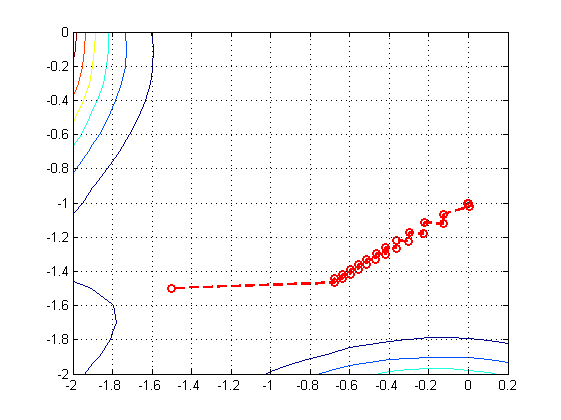
\includegraphics[width=3.4in]{figures/2d2-steepestDescent.png}
\caption{Steepest Descent}
\label{figSD2}
\end{figure}

%%%%%%%%%%%%%%%%%%%%%%%%%%%%%%%%%%%%%%%%%%%%%%%%%%%%%%%%%%%%%%%%%%%%%%%%%%%%%%%%
\subsection{Quasi-Newton Method}

Lastly, the Quasi-Newton method was implemented to search for the minimum of the Goldstein-Price function. This method was implemented with the BFGS approximation for the Hessian matrix.

This method seemed to have the opposite performance than arbitrary line search. It was a very unstable method, especially coupled with the uncertainty of the Brent's method 1D minimizer. When this method converged to the global minimum, as shown in Fig. \ref{figQN}, it did so in few iterations, but this result was not common when applied on the Goldstein-Price function. This specific run took 8 iterations to reach the global minimum starting from $(x,y) = (0,0)$.

\begin{figure}[H]
\centering
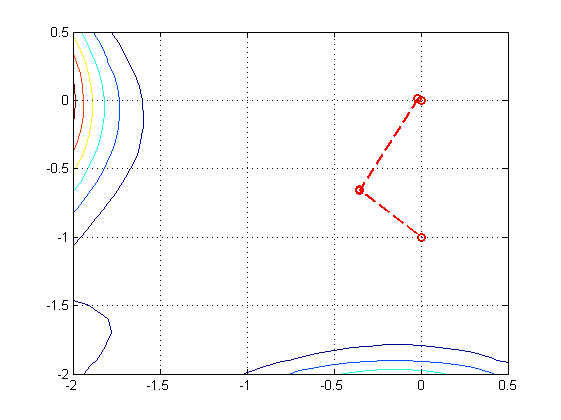
\includegraphics[width=3.4in]{figures/2d2-quasiNewton.png}
\caption{Quasi-Newton Method}
\label{figQN}
\end{figure}

These results suggest there is a trade-off between speed of convergence and stability of an optimization method. This should be taken into account when trying to minimize a function in a real application, with the best choice bing stable methods such as arbitrary line search for functions that are expected to have highly erratic behaviours.


%%%%%%%%%%%%%%%%%%%%%%%%%%%%%%%%%%%%%%%%%%%%%%%%%%%%%%%%%%%%%%%%%%%%%%%%%%%%%%%%
%%%%%%%%%%%%%%%%%%%%%%%%%%%%%%%%%%%%%%%%%%%%%%%%%%%%%%%%%%%%%%%%%%%%%%%%%%%%%%%%
\section{Minimization In nD}

In this part we attempted to determine the ellipse that best fitted a set of noisily sampled random points from a shape of elliptical nature. The math for the ellipses used the parametric representation of a translated and rotated ellipse. The ellipse was defined by five parameters:

\begin{itemize}
    \item $a$ - Radius of the ellipse in the direction $\phi$
    \item $b$ - Radius of the ellipse in the direction perpendicular to $\phi$
    \item $xc$ - x component of the center position
    \item $yc$ - y component of the center position
    \item $\phi$ - Angle of rotation of the ellipse
\end{itemize}

The parametric equations used for describing an ellipse with these parameters are Eqs. \ref{el1} and \ref{el2}, where $\theta \in [0,2\pi]$

\begin{equation}
x(\theta) = xc + a*cos(\theta)cos(\phi) - b*sin(\theta)sin(\phi)
\label{el1}
\end{equation}

\begin{equation}
y(\theta) = yc + a*cos(\theta)sin(\phi) + b*sin(\theta)cos(\phi)
\label{el2}
\end{equation}

The first step was to generate a noisy set of samples of an ellipse. The chosen parameters were: $a=5$, $b=3$, $xc = 1$, $yc = 1$, and $\phi = \pi /4$. A set of 500 points generated according to these parameters to these parameters can be seen in Fig. \ref{figGT}.


\begin{figure}[H]
\centering
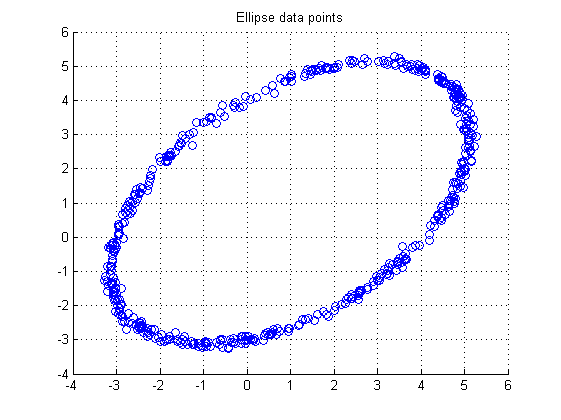
\includegraphics[width=3.4in]{figures/nd-groundTruth.png}
\caption{Noisy sampling of points belonging to the given ellipse}
\label{figGT}
\end{figure}

The next step was to develop a cost function for each point. This is the function whose sum would be minimized to fit the ellipse. The chosen function followed two steps: 

\begin{itemize}
    \item Find out the angle from the ellipse center towards the current point
    \item Calculate the distance between the current point and the ideal point given the current parameters
\end{itemize}

This function is a basic function that approaches zero as the estimated parameters approach the real parameters of the sampled ellipse.

Next, the Levenberg-Marquardt method was used to minimize the function F, which is half of the sum of the cost function at all sampled points for the current estimated parameters. Since our cost function only had one output, the Jacobian could be calculated using the gradient function used in the previous sections.

Figure \ref{figFE} shows the result of the Levenberg-Marquardt method after being applied to the points showed in Fig. \ref{figGT}. It can be observed that the fitted ellipse is slightly more round than the sampled ellipse. This occurs because we used a simple cost function, and it could probably be ficed by using a more elaborate cost function to be minimized by this method.

The application of the Levenberg-Marquardt method showed in Fig. \ref{figFE} took 101 iterations to converge. The number of iterations to reach convergence varied depending on the set of points that was generated, but most tries converged in 100 to 300 iterations. It's also important that this method was not observed to diverge or to obtain a wrong result. The inly variation in the result was due to the fact that the same ellipse can be defined by two sets of parameters, that is, if $\phi _2 = \phi _1 \pm \pi/2$, and $a_2 = b_1$, and $b_2 = a_1$, both sets of parameters define the same ellipse.

The parameters estimated by the Levenberg-Marquardt method as showed in \ref{figFE} were: $a=4.4668$, $b=3.4353$, $xc=0.9883$, $yc=0.9998$, $\phi = 0.7933$.

\begin{figure}[H]
\centering
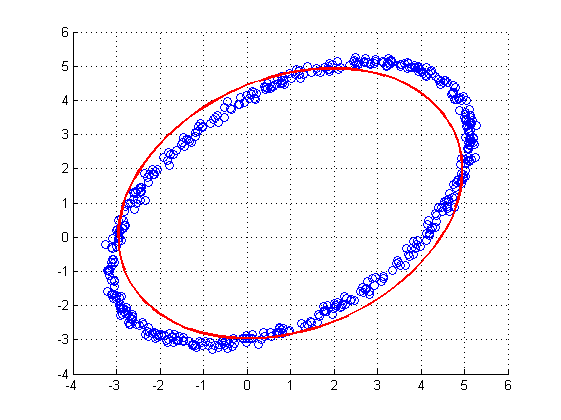
\includegraphics[width=3.4in]{figures/nd-fittedEllipse.png}
\caption{Result of best fitting ellipse}
\label{figFE}
\end{figure}


%%%%%%%%%%%%%%%%%%%%%%%%%%%%%%%%%%%%%%%%%%%%%%%%%%%%%%%%%%%%%%%%%%%%%%%%%%%%%%%%
%%%%%%%%%%%%%%%%%%%%%%%%%%%%%%%%%%%%%%%%%%%%%%%%%%%%%%%%%%%%%%%%%%%%%%%%%%%%%%%%
\section{Conclusion}

Several function optimization methods were demonstrated. Each of these methods seems to have a different application, and each method's advantages and disadvantages should be taken into account when choosing the best optimization method for a given application.

The most important conclusion to be taken from the observation of all these different optimization methods is that there seems to be a trade-off between the speed of convergence of an optimization method and its stability aand this should be taken into account when choosing the optimization method to be implemented.


%%%%%%%%%%%%%%%%%%%%%%%%%%%%%%%%%%%%%%%%%%%%%%%%%%%%%%%%%%%%%%%%%%%%%%%%%%%%%%%%
%%%%%%%%%%%%%%%%%%%%%%%%%%%%%%%%%%%%%%%%%%%%%%%%%%%%%%%%%%%%%%%%%%%%%%%%%%%%%%%%
\bibliographystyle{IEEEtran}
\bibliography{references}

%%%%%%%%%%%%%%%%%%%%%%%%%%%%%%%%%%%%%%%%%%%%%%%%%%%%%%%%%%%%%%%%%%%%%%%%%%%%%%%%
%%%%%%%%%%%%%%%%%%%%%%%%%%%%%%%%%%%%%%%%%%%%%%%%%%%%%%%%%%%%%%%%%%%%%%%%%%%%%%%%
\appendices

%\begin{figure*}[p]
%\section{Code}
%Appendix one text goes here.
%\end{figure*}




% that's all folks
\end{document}


